\documentclass[sigconf]{acmart}
\AtBeginDocument{%
  \providecommand\BibTeX{{%
    Bib\TeX}}}

\usepackage{lipsum}
\usepackage{algorithm}
\usepackage{algpseudocode} 
\usepackage{amsmath}
\usepackage{placeins}
\usepackage{cleveref}
\usepackage{multirow}
\usepackage{booktabs}
\usepackage{enumitem}
\usepackage{url}
\setcopyright{acmlicensed}
\copyrightyear{2018}
\acmYear{2018}
\acmDOI{XXXXXXX.XXXXXXX}
\acmConference[Conference acronym 'XX]{Make sure to enter the correct
  conference title from your rights confirmation email}{June 03--05,
  2018}{Woodstock, NY}

\acmISBN{978-1-4503-XXXX-X/2018/06}

\begin{document}

\title{Report}

\author{\textcolor{blue}{---}}
\affiliation{%
  \institution{---}
  \country{South Korea}
}
\email{---}

\renewcommand{\shortauthors}{\textcolor{blue}{Kim et al.}}



\settopmatter{printacmref=false} % Removes citation block in the first page
\renewcommand\footnotetextcopyrightpermission[1]{} % Removes footnote with conference info



\maketitle


\section{INTRODUCTION}
Various tree structures are used for implementing the efficient indexing in the database in many systems.
In this report, we implemented three tree data structures (B-Tree, B$^+$-Tree, B*-Tree) used for database indexing.
Also, we conducted a integrity check and various timing benchmarks for insert, lookup, range operation, and erase with different order of the trees.

Throughout this report we follow the CLRS\cite{Cormen_Leiserson_Rivest_Stein_2022} minimum-degree convention $t$, where a non-root node holds between $t - 1$ and $2t - 1$ keys. 
Our implementation exposes the fan-out order $d$ (Knuth's convention, the maximum number of children per node) as the configurable external parameter, and internally converts it to $t=\left\lceil \frac{d}{2} \right\rceil$. 
Because CLRS's parameterization can only express even fan-outs ($d = 2t$), an odd input $d$ rounds up to $d + 1$ (e.g., $d=5$ yields $t = 3$ with effective max children 6). 
Throughout the experiments, the reported tree order $d$ corresponds to an internal minimum degree of $t = \lceil d/2 \rceil$.

\section{Fundamental Index Structure (B-tree)}
\subsection{B-Tree}
\label{sec:btree}
A B-tree is a tree data structure that have following properties\cite{Cormen_Leiserson_Rivest_Stein_2022}:
\begin{itemize}[noitemsep, topsep=0pt, parsep=0pt, partopsep=0pt]
    \item Each node $x$ have a $x.n$ keys and the key is stored in monotonically increasing order.
    \item Each internal node $x$ have $x.n + 1$ pointers to its children.
    \item The $i$-th key of the node $x$ $x.key_{i}$ separate the ranges of keys stored in each subtree: if $k_{i}$ is any key stored in the subtree with root $i$-th child of $x$, 
    then $k_{1} \le x.key_{1} \le k_{2} \le x.key_{2} \le \dots \le x.key_{x.n} \le k_{x.n+1}$
    \item All leaves have the same depth.
    \item There is a $t$ for tree which indicates the minimum degree of the tree.
    \begin{itemize}[noitemsep, topsep=0pt, parsep=0pt, partopsep=0pt]
      \item Every node other than the root must have at least $t - 1$ keys. Therefore all internal nodes other than the root should have at least $t$ children.
      \item Every node may contain at most $2t - 1$ keys. Therefore, an internal node may have at most $2t$ children.
    \end{itemize}
\end{itemize}

\subsubsection{Search}
The \textit{Search} operation finds the key in the node which is greater or equal to the target key and if the key is not equal, goes to the child node and do \textit{Search} recursively. The pseudocode is given in \Cref{alg:btree-search}.

\begin{algorithm}[tbp]
\caption{B-Tree Search Algorithm}
\label{alg:btree-search}
\begin{algorithmic}[1]
\Procedure{Search}{$node, key$}
    \State $i \gets 0$
    \While{$i < |node.keys|$ \textbf{and} $key > node.keys[i]$}
        \State $i \gets i + 1$
    \EndWhile
    \If{$i < |node.keys|$ \textbf{and} $key = node.keys[i]$}
        \State \Return $(node, i)$
    \EndIf
    \If{$node.is\_leaf$}
        \State \Return \text{NIL}
    \EndIf
    \State \Return \Call{Search}{$node.children[i], key$}
\EndProcedure
\end{algorithmic}
\end{algorithm}

\subsubsection{Insert}
\textit{Insert} performs the same descent as \textit{Search}, but preemptively invokes \textit{Split-Child} whenever the child it is about to descend into is full ($2t-1$ keys); this guarantees \textsc{Insert-Nonfull} never recurses into a node that cannot accommodate one more key. The root, having no parent, is handled separately: a full root is wrapped in a new internal node and split, which is the only mechanism by which a B-tree grows in height. \Cref{alg:btree-insert} shows the procedure. 

\begin{algorithm}[tbp]
\caption{B-Tree Insert Algorithm}
\label{alg:btree-insert}
\begin{algorithmic}[1]
\Procedure{Insert}{$T, key, value$}
    \If{$T.root = NIL$}
        \State $T.root \gets$ \text{new leaf node with} $(key, value)$; \Return
    \EndIf
    \If{$|T.root.keys| = 2t - 1$}
        \State $new\_root \gets$ \text{new internal node}
        \State $new\_root.children.push\_back(T.root)$
        \State \Call{Split-Child}{$new\_root, 0$}
        \State $T.root \gets new\_root$
    \EndIf
    \State \Return \Call{Insert-Nonfull}{$T.root, key, value$}
\EndProcedure
\Statex
\Procedure{Insert-Nonfull}{$node, key, value$}
    \State $i \gets$ \text{index of key in node}
    \If{$i < |node.keys|$ \textbf{and} $key = node.keys[i]$}
        \State $node.values[i] \gets value$; \Return
    \EndIf
    \If{$node.is\_leaf$}
        \State \text{Insert} $(key, value)$ \text{at position} $i$; \Return
    \EndIf
    \If{$|node.children[i].keys| = 2t - 1$}
        \State \Call{Split-Child}{$node, i$}
        \If{$key > node.keys[i]$} \State $i \gets i + 1$ \EndIf
    \EndIf
    \State \Return \Call{Insert-Nonfull}{$node.children[i], key, value$}
\EndProcedure
\Statex
\Procedure{Split-Child}{$parent, i$}
    \State $full\_node \gets parent.children[i]$
    \State $sibling \gets$ \text{new node with same} $is\_leaf$ \text{value}
    \State $sibling.keys \gets full\_node.keys[t .. 2t - 2]$
    \State $sibling.values \gets full\_node.values[t .. 2t - 2]$
    \If{$not \: full\_node.is\_leaf$}
        \State $sibling.children \gets full\_node.children[t .. 2t - 1]$
    \EndIf
    \State $mid\_k \gets full\_node.keys[t - 1]$
    \State $mid\_v \gets full\_node.values[t - 1]$
    \State \text{truncate full\_node to its left half}
    \State \text{insert sibling into} $parent.children[i+1]$
    \State \text{insert} $(mid\_k, mid\_v)$ \text{into} $parent$ \text{at} $i$
\EndProcedure
\end{algorithmic}
\end{algorithm}

\subsubsection{Erase}
The \textit{Erase} operation finds the key by descending the tree similar to \textit{Search}. 
The action depends on where the key is found and the cardinality of the relevant child:
\begin{itemize}[noitemsep, topsep=0pt, parsep=0pt, partopsep=0pt]
    \item \textbf{Key in a leaf node}: simply remove the (key, value) pair from the leaf.
    \item \textbf{Key in an internal node}, left child has $\ge$ t keys: replace the key with its in-order predecessor (the rightmost key in the left subtree), then recursively erase that predecessor from the left subtree.
    \item \textbf{Key in an internal node, right child has $\ge$ t keys}: symmetric to above, using the in-order successor.
    \item \textbf{Key in an internal node, both children at exactly $t - 1$ keys}: merge the two children together with the separator key (forming a single child with $2t - 1$ keys), then recursively erase from the merged child.
    \item \textbf{Key not in the current node}: descend into the appropriate child. Before descent, if that child has $\le$ $t - 1$ keys, call Fill to bring it to $\ge$ $t$ keys (by Rotate-Right, Rotate-Left, or Merge-Two with a sibling). This pre-condition mirrors the preemptive Split in Insert: the parent ensures the descended child can survive one more deletion without violating the $t - 1$ minimum.
\end{itemize}
The full procedure is given in \Cref{alg:btree-erase}.

\begin{algorithm}[tbp]
\caption{B-Tree Erase Algorithm}
\label{alg:btree-erase}
\begin{algorithmic}[1]
\Procedure{Erase}{$T, key$}
    \If{$T.root = \text{NIL}$} \State \Return \EndIf
    \State \Call{Do-Erase}{$T.root, key$}
    \If{$|T.root.keys| = 0$}
        \State $old \gets T.root$
        \If{$old.is\_leaf$} \State $T.root \gets \text{NIL}$
        \Else \State $T.root \gets old.children[0]$
        \EndIf
        \State \text{free } $old$
    \EndIf
\EndProcedure
\Statex
\Procedure{Do-Erase}{$node, key$}
    \State $i \gets$ \text{index of key in node}
    \If{$i < |node.keys|$ \textbf{and} $key = node.keys[i]$}
        \If{$node.is\_leaf$}
            \State \text{remove } $(node.keys[i], node.values[i])$
        \Else
            \State \Call{Erase-Internal}{$node, i$}
        \EndIf
        \State \Return
    \EndIf
    \If{$node.is\_leaf$} \State \Return \EndIf
    \State $last \gets (i = |node.keys|)$
    \If{$|node.children[i].keys| \le t - 1$}
        \State \Call{Fill}{$node, i$}
    \EndIf
    \If{$last$ \textbf{and} $i > |node.keys|$}
        \State \Call{Do-Erase}{$node.children[i - 1], key$}; \Return
    \EndIf
    \State \Call{Do-Erase}{$node.children[i], key$}
\EndProcedure
\Statex
\Procedure{Erase-Internal}{$node, i$}
    \State $L \gets node.children[i]$;\quad $R \gets node.children[i+1]$
    \If{$|L.keys| \ge t$}
        \State $(k, v) \gets$ \text{rightmost (key, value) in } $L$
        \State $node.keys[i] \gets k$;\quad $node.values[i] \gets v$
        \State \Call{Do-Erase}{$L, k$}
    \ElsIf{$|R.keys| \ge t$}
        \State $(k, v) \gets$ \text{leftmost (key, value) in } $R$
        \State $node.keys[i] \gets k$;\quad $node.values[i] \gets v$
        \State \Call{Do-Erase}{$R, k$}
    \Else
        \State $key \gets node.keys[i]$
        \State \Call{Merge-Two}{$node, i$}
        \State \Call{Do-Erase}{$node.children[i], key$}
    \EndIf
\EndProcedure
\Statex
\Procedure{Fill}{$parent, i$}
    \If{$i > 0$ \textbf{and} $|parent.children[i-1].keys| \ge t$}
        \State \Call{Rotate-Right}{$parent, i$}
    \ElsIf{$i < |parent.keys|$ \textbf{and} $|parent.children[i+1].keys| \ge t$}
        \State \Call{Rotate-Left}{$parent, i$}
    \Else
        \If{$i < |parent.keys|$} \State \Call{Merge-Two}{$parent, i$}
        \Else \State \Call{Merge-Two}{$parent, i-1$}
        \EndIf
    \EndIf
\EndProcedure
\end{algorithmic}
\end{algorithm}
\FloatBarrier
\subsubsection{Range Query}
The \textit{Range} operation performs an in-order traversal bounded by $[low, high]$, descending into a child's subtree before visiting each key whose value falls in the range. \Cref{alg:btree-range} gives the pseudocode.

\begin{algorithm}[tbp]
\caption{B-Tree Range Query}
\label{alg:btree-range}
\begin{algorithmic}[1]
\Procedure{Range}{$node, low, high, visit$}
    \State $i \gets 0$
    \While{$i < |node.keys|$ \textbf{and} $node.keys[i] < low$}
        \State $i \gets i + 1$
    \EndWhile
    \While{$i < |node.keys|$ \textbf{and} $node.keys[i] \le high$}
        \If{\textbf{not} $node.is\_leaf$}
            \State \Call{Range}{$node.children[i], low, high, visit$}
        \EndIf
        \State \Call{Visit}{$node.keys[i], node.values[i]$}
        \State $i \gets i + 1$
    \EndWhile
    \If{\textbf{not} $node.is\_leaf$}
        \State \Call{Range}{$node.children[i], low, high, visit$}
    \EndIf
\EndProcedure
\end{algorithmic}
\end{algorithm}

\section{Advanced Index Structure (B+-tree, B*-tree)}
\subsection{B$^+$-Tree}
A B$^+$-tree shares the structural invariants of a B-tree (\Cref{sec:btree}) but differs in two key ways: (1) all satellite data (record pointers) is stored only in leaf nodes, while internal nodes hold only routing keys; and (2) leaf nodes are linked as a doubly-linked list to support efficient sequential access. Internal-node routing uses strict inequalities --- if $k$ is in the subtree of the $i$-th child then $k < x.key_i$, and equal keys descend to the right.

\subsubsection{Search}
Since B$^+$-Tree contains the data only in the leaf nodes, it first finds the leaf node contains the key and search the leaf node iteratively. The pseudocode is given in \Cref{alg:bplus-search}.

\begin{algorithm}[tbp]
\caption{B+ Tree Search Algorithm}
\label{alg:bplus-search}
\begin{algorithmic}[1]
\Procedure{Search}{$T, key$}
    \State $leaf \gets \Call{Find-Leaf}{T.root, key}$
    \State $i \gets$ \text{first index such that } $leaf.keys[i] \ge key$
    \If{$i < |leaf.keys|$ \textbf{and} $leaf.keys[i] = key$}
        \State \Return $(leaf, i)$
    \EndIf
    \State \Return \text{NIL}
\EndProcedure
\end{algorithmic}

\begin{algorithmic}[1]
\Procedure{Find-Leaf}{$node, key$}
    \While{\textbf{not} $node.is\_leaf$}
        \State $i \gets$ \text{first index such that } $key < node.keys[i]$
        \State $node \gets node.children[i]$
    \EndWhile
    \State \Return $node$
\EndProcedure
\end{algorithmic}
\end{algorithm}

\subsubsection{Insert}

The \textit{Insert} operation of the B$^+$-Tree have the same method as B-Tree (\Cref{alg:btree-insert}).
However, the \textit{Split} for leaf node is little different. It doesn't remove the mid key from the leaf node.
Instead, it copied from the leaf node to parent node and serve as router in the parent node.
\textit{Split} for internal node is same as the normal B-Tree. The leaf split procedure is shown in \Cref{alg:bplus-insert}.

\begin{algorithm}[tbp]
\caption{B+ Tree Insert Algorithm}
\label{alg:bplus-insert}
\begin{algorithmic}[1]
\Procedure{Split-Leaf-Child}{$parent, i$}
    \State $full\_node \gets parent.children[i]$
    \State $sibling \gets$ \textbf{new} leaf node

    \State $sibling.keys \gets full\_node.keys[t \dots 2t-1]$
    \State $sibling.values \gets full\_node.values[t \dots 2t-1]$
    
    \State \text{truncate } $full\_node$ \text{ to first } $t$ \text{ keys}
    \State \Call{Link-Leaf-List}{$full\_node, sibling$}
    
    \State $router \gets sibling.keys[0]$
    \State \text{insert } $sibling$ \text{ into } $parent.children$ \text{ at position } $i+1$
    \State \text{insert } $router$ \text{ into } $parent.keys$ \text{ at position } $i$
\EndProcedure


\Procedure{Split-Internal-Child}{$parent, i$}
    \State \Comment{Same logic with Split-Child in B-Tree}
\EndProcedure
\end{algorithmic}
\end{algorithm}

\subsubsection{Erase}

The \textit{Erase} method follows the same logic as B-Tree, but with two simplifications: actual key removal only occurs at leaf nodes, and the case-analysis of B-tree's \textsc{Erase-Internal} is unnecessary because internal keys are mere routing copies. Stale internal routing keys are tolerated since they still correctly partition the subtrees. \textsc{Merge-Two} is identical to B-tree's, except that when merging two leaves it additionally updates the leaf-list pointer ($L.next \gets R.next$). \Cref{alg:bplus-erase} shows the modified \textsc{Do-Erase}.

\begin{algorithm}[tbp]
\caption{B+ Tree Erase Algorithm}
\label{alg:bplus-erase}
\begin{algorithmic}[1]
\Procedure{Do-Erase}{$node, key$}
    \If{$node.is\_leaf$}
        \If{$key$ \text{ is found in } $node$}
            \State \text{remove } $(key, value)$
        \EndIf
        \State \Return
    \EndIf
    \State $i \gets$ \text{first index such that } $key < node.keys[i]$
    \If{$|node.children[i].keys| \le t - 1$}
        \State $i \gets \Call{Fill}{node, i}$
    \EndIf
    \State \Call{Do-Erase}{$node.children[i], key$}
\EndProcedure
\end{algorithmic}
\end{algorithm}

\subsubsection{Range}

Since B$^+$-Tree have a links between leaf nodes and actual data is only contained in the leaf nodes, the \textit{Range} leverages this property.
\textit{Range} operation finds the leaf node with the low key and iteratively traverse the leaf nodes instead of in-order traversal in B-Tree. The pseudocode is given in \Cref{alg:bplus-range}.

\begin{algorithm}[tbp]
\caption{B+ Tree Range Query}
\label{alg:bplus-range}
\begin{algorithmic}[1]
\Procedure{Range}{$T, low, high, visit$}
    \State $leaf \gets \Call{Find-Leaf}{T.root, low}$
    \State $i \gets$ \text{first index such that } $leaf.keys[i] \ge low$
    \While{$leaf \neq \text{NIL}$}
        \For{$j \gets i$ \textbf{to} $|leaf.keys| - 1$}
            \If{$leaf.keys[j] > high$}
                \State \Return
            \EndIf
            \State \Call{Visit}{$leaf.keys[j], leaf.values[j]$}
        \EndFor
        \State $leaf \gets leaf.next$
        \State $i \gets 0$
    \EndWhile
\EndProcedure
\end{algorithmic}
\end{algorithm}


\subsection{B*-Tree}
A B*-tree is a variant of the B-tree introduced by Knuth\cite{knuth1998} that aims for higher average node occupancy. While a standard B-tree guarantees $\ge t-1$ keys per non-root node ($\approx 1/2$ full), a B*-tree targets approximately $2/3$ occupancy by deferring splits.

\subsubsection{Insert Policy}
A B*-tree shares the same structural invariants as a B-tree (same capacity, leaf-depth, routing semantics); only the split policy on insertion differs. When a child becomes full, the algorithm first attempts \textbf{cooperative redistribution}: if an adjacent sibling has spare capacity, keys are redistributed between them and the parent's separator is updated, allocating no new node. Only when both adjacent siblings are also full does the algorithm fall back to a \textbf{$2 \to 3$ split}: the full child and one full sibling (a combined $4t - 3$ keys including the separator) are repartitioned into three nodes of approximately $\lceil (4t-3)/3 \rceil$ keys each, promoting two new separators. Newly created nodes thus start at $\approx 2/3$ capacity instead of B-tree's $1/2$. \Cref{alg:bstar-split} shows the modified \textsc{Do-Split}; \textsc{Redistribute-With-Left} is the symmetric mirror of \textsc{Redistribute-With-Right} and is omitted.

\subsubsection{Erase Policy}
Maintaining a strict $2/3$ minimum on \textit{erase} would require a $3 \to 2$ merge mechanism that is mathematically impossible at certain corner cases (e.g., a non-leaf root with two children both at the strict minimum, whose combined size exceeds capacity). Real-world implementations such as HFS+ and NTFS therefore fall back to B-tree's erase semantics, and we follow the same practical choice: \textit{Erase}, \textit{Erase-Internal}, and \textit{Fill} are inherited unchanged from B-tree (\Cref{alg:btree-erase}). The $\approx 2/3$ occupancy is thus a statistical tendency from insertions, not a strict invariant maintained on deletion.

\begin{algorithm}[tbp]
\caption{B* Tree Split and Redistribution}
\label{alg:bstar-split}
\begin{algorithmic}[1]
\Procedure{Do-Split}{$parent, i$}
    \State $M \gets 2t - 1$
    \If{$i > 0$ \textbf{and} $|parent.children[i-1].keys| \le M - 2$}
        \State \Call{Redistribute-With-Left}{$parent, i$}
        \State \Return
    \ElsIf{$i < |parent.keys|$ \textbf{and} $|parent.children[i+1].keys| \le M - 2$}
        \State \Call{Redistribute-With-Right}{$parent, i$}
        \State \Return
    \EndIf
    
    \If{$i < |parent.keys|$}
        \State \Call{Split-Two-Into-Three}{$parent, i$}
    \ElsIf{$i > 0$}
        \State \Call{Split-Two-Into-Three}{$parent, i - 1$}
    \Else
        \State \Call{Split-In-Two}{$parent, i$}
    \EndIf
\EndProcedure

\Procedure{Redistribute-With-Right}{$parent, i$}
    \State $L \gets parent.children[i]$
    \State $R \gets parent.children[i+1]$
    \State $K \gets L.keys \mathbin{++} [parent.keys[i]] \mathbin{++} R.keys$
    \State $V \gets$ \text{analogous for values}
    
    \State $new\_L \gets \lfloor |K| / 2 \rfloor$
    
    \State $L.keys, L.values \gets K[0 \dots new\_L - 1]$
    \State $parent.keys[i], parent.values[i] \gets K[new\_L]$
    \State $R.keys, R.values \gets K[new\_L + 1 \dots]$
    \State \Comment{Children pointers redistributed analogously when not leaves}
\EndProcedure
\end{algorithmic}
\end{algorithm}

\addtocounter{algorithm}{-1}
\begin{algorithm}[tbp]
\caption{B* Tree Split and Redistribution (Continued)}
\begin{algorithmic}[1]
\Procedure{Split-Two-Into-Three}{$parent, i$}
    \State $L \gets parent.children[i]$
    \State $R \gets parent.children[i+1]$
    \State $K \gets L.keys \mathbin{++} [parent.keys[i]] \mathbin{++} R.keys$
    \State $V \gets$ \text{analogous for values}
    
    \State $keys\_to\_distribute \gets |K| - 2$
    \State $a \gets \lceil keys\_to\_distribute / 3 \rceil$
    \State $b \gets \lceil (keys\_to\_distribute - a) / 2 \rceil$
    
    \State $M\_node \gets$ \textbf{new} node
    \State $L.keys \gets K[0 \dots a - 1]$
    \State $sep1 \gets K[a]$
    \State $M\_node.keys \gets K[a + 1 \dots a + b]$
    \State $sep2 \gets K[a + b + 1]$
    \State $R.keys \gets K[a + b + 2 \dots]$
    
    \State $parent.keys[i] \gets sep1$
    \State \text{insert } $sep2$ \text{ into } $parent.keys$ \text{ at position } $i+1$
    \State \text{insert } $M\_node$ \text{ into } $parent.children$ \text{ at position } $i+1$
\EndProcedure
\end{algorithmic}
\end{algorithm}

\subsection{Time Complexity Comparison}
For all three trees, the height is $O(\log_t n)$ and per-node key search is $O(t)$ (linear) or $O(\log t)$ (binary), giving Search/Insert/Erase costs of $O(t \log_t n)$ or $O(\log n)$ respectively. The B$^+$-tree's Search always descends to a leaf even when an internal routing key matches, which adds only a constant factor. Range queries cost $O(\log_t n + k)$ asymptotically for all three; however, the B$^+$-tree leaf-list scan touches $\lceil k/B \rceil$ contiguous nodes (where $B$ is leaf occupancy), whereas the B-tree and B*-tree in-order recursion additionally visits $O(k/t)$ internal nodes --- a constant-factor advantage for B$^+$-tree on cache- or disk-bound workloads. The B*-tree Insert keeps the same asymptotic bound, but each split on the path performs cooperative redistribution or $2 \to 3$ split at a $\Theta(t)$ cost --- roughly a $2$--$3\times$ constant-factor overhead compared to B-tree's simple $1 \to 2$ split, traded for higher fill factor.

\section{Experimental Results and Analysis}
\subsection{Experiment Setup}
We run the insertion of $100000$ datas in given csv file into the tree and indexing of $100000$ keys, which is consists of inserted key in the given data and random keys that may not be in the data.
Also, we run the range operations in various range sizes where it calculates the sum of the 1000x of the GPA of all students in given range.
Morever, we performed the erase of $50000$ random keys in the tree.
During the erase, it checks whether the tree violates the property of the trees such as node key size and same height prooperty.
We used a average data of 10 repetitions. To remove a difference caused by the cache and other system issues, we run the 2 times of workload before the actual run.
The environment is WSL2 on the Windows 11 with Intel(R) Core(TM) Ultra 7 258V CPU and 16GB RAM.
The code is compiled with -std=c++17 -fsanitize=address -O2 flags.
The raw data in text and csv form and implementation code is available at GitHub repository: \url{https://github.com/YOUR_USERNAME/YOUR_REPOSITORY_NAME}.

\subsection{Insertion and Parameter Tuning}

\begin{figure}[H]
  \centering
  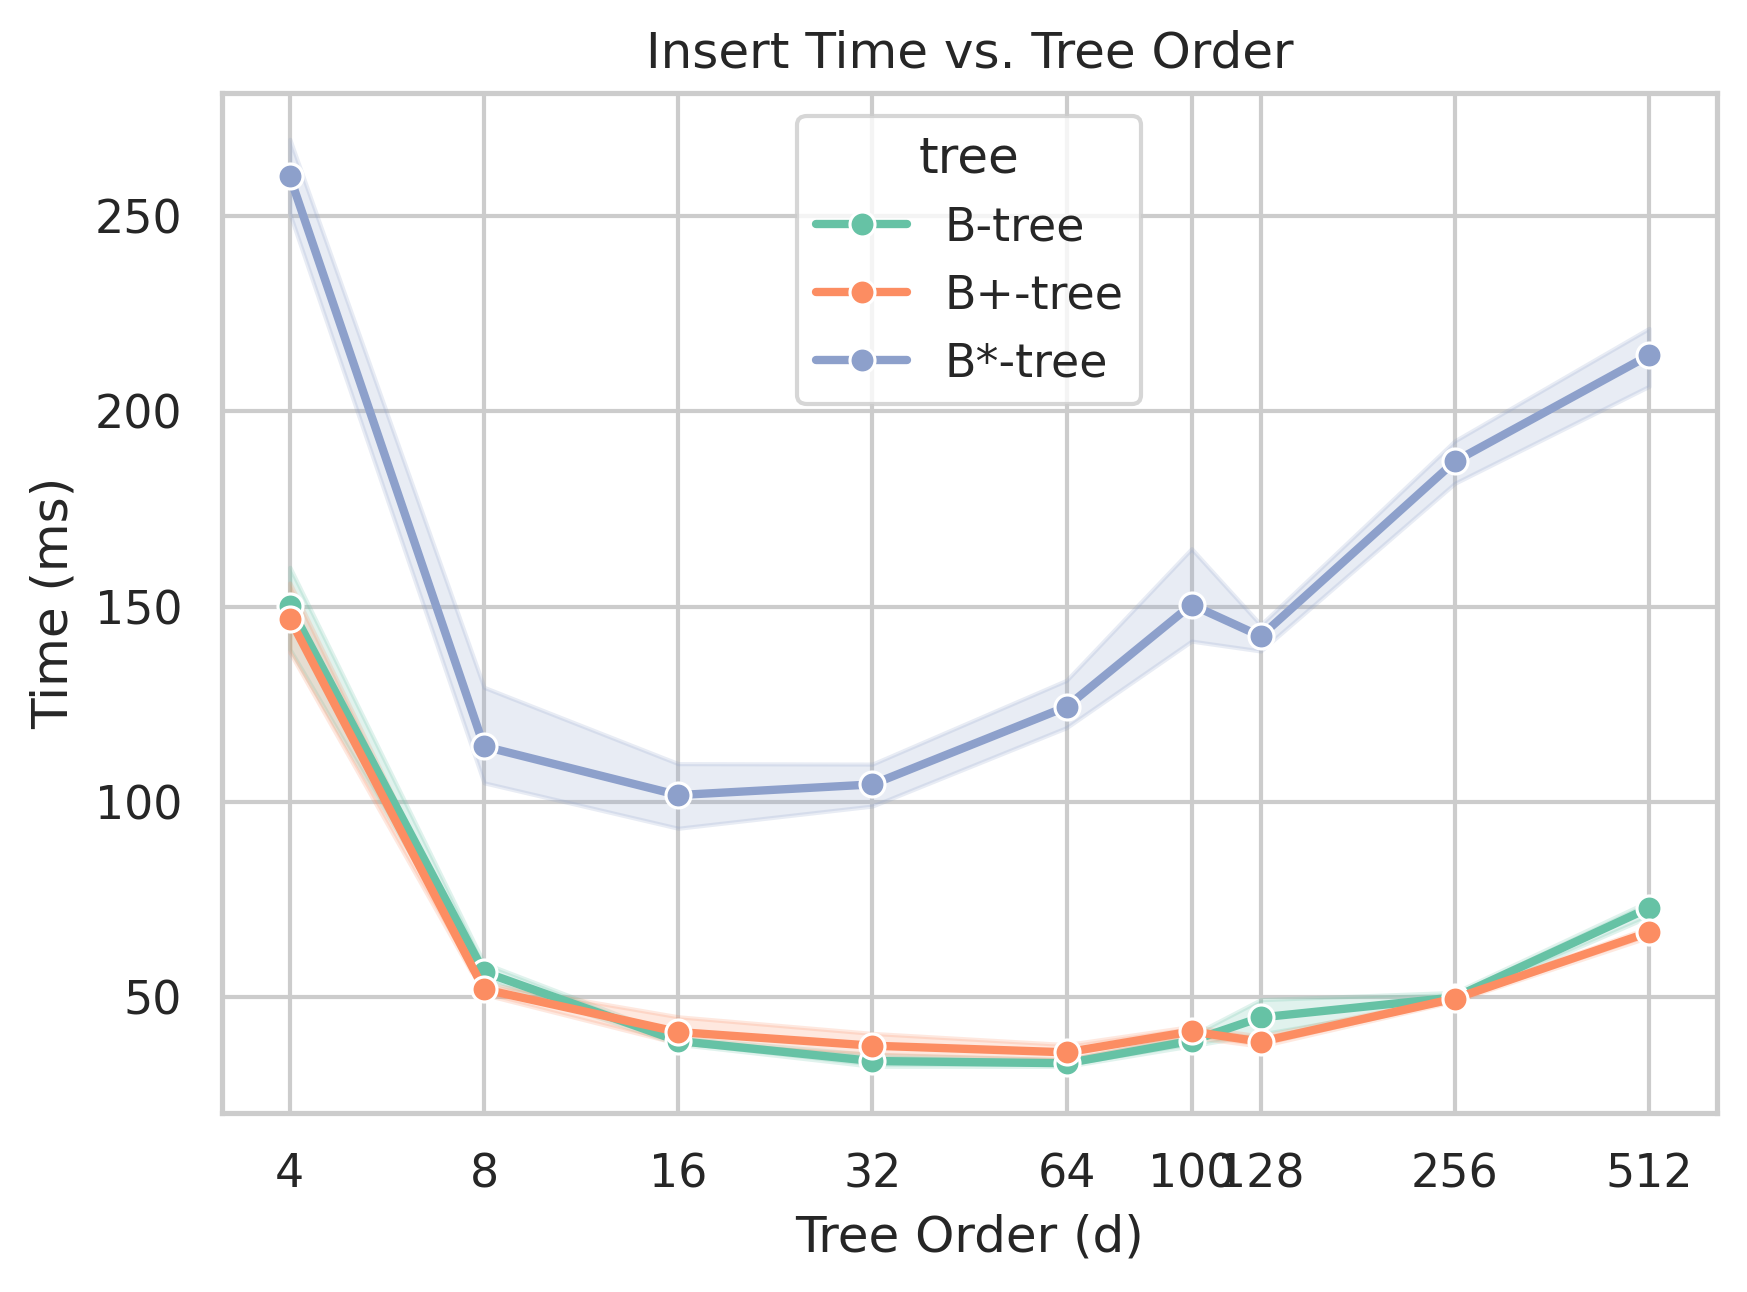
\includegraphics[width=0.7\linewidth]{figure/perf_insert.png}
  \caption{Performance graph for inserting 100000 datas}
  \label{fig:perf_insert}
\end{figure}

As shown in \cref{fig:perf_insert}, for the insertion, B*-Tree shows the worst performance in all orders.
B-Tree and B+-Tree shows a insignificant differences on ther performance.
With the respect to the orders, the performance is increasing as the order grows until the order reaches at some point around 100, after which the performance decreases.

Unlike B-tree and B$^+$-tree, which perform a simple $1 \to 2$ node split upon overflow, the B*-tree delays the split by attempting to redistribute keys to adjacent siblings to maintain a $2/3$ minimum occupancy. 
If the siblings are also full, it performs a complex $2 \to 3$ split, which causes significant memory copy overhead and frequent cache misses during the insertion phase.

The U-shaped performance curve across different orders illustrates the trade-off between tree height and intra-node operations.
As the order $d$ increases up to approximately 100, the tree height $O(\log_d n)$ decreases logarithmically.  
However, as the order continues to grow beyond the sweet spot ($d > 100$), the size of the internal sorted arrays becomes excessively large.
Inserting the keys in such large nodes causes many memory move overhead, which overshadows the benefits of a shallower tree, leading to performance drop.

\subsection{Indexing and Parameter Tuning}
\begin{figure}[H]
  \centering
  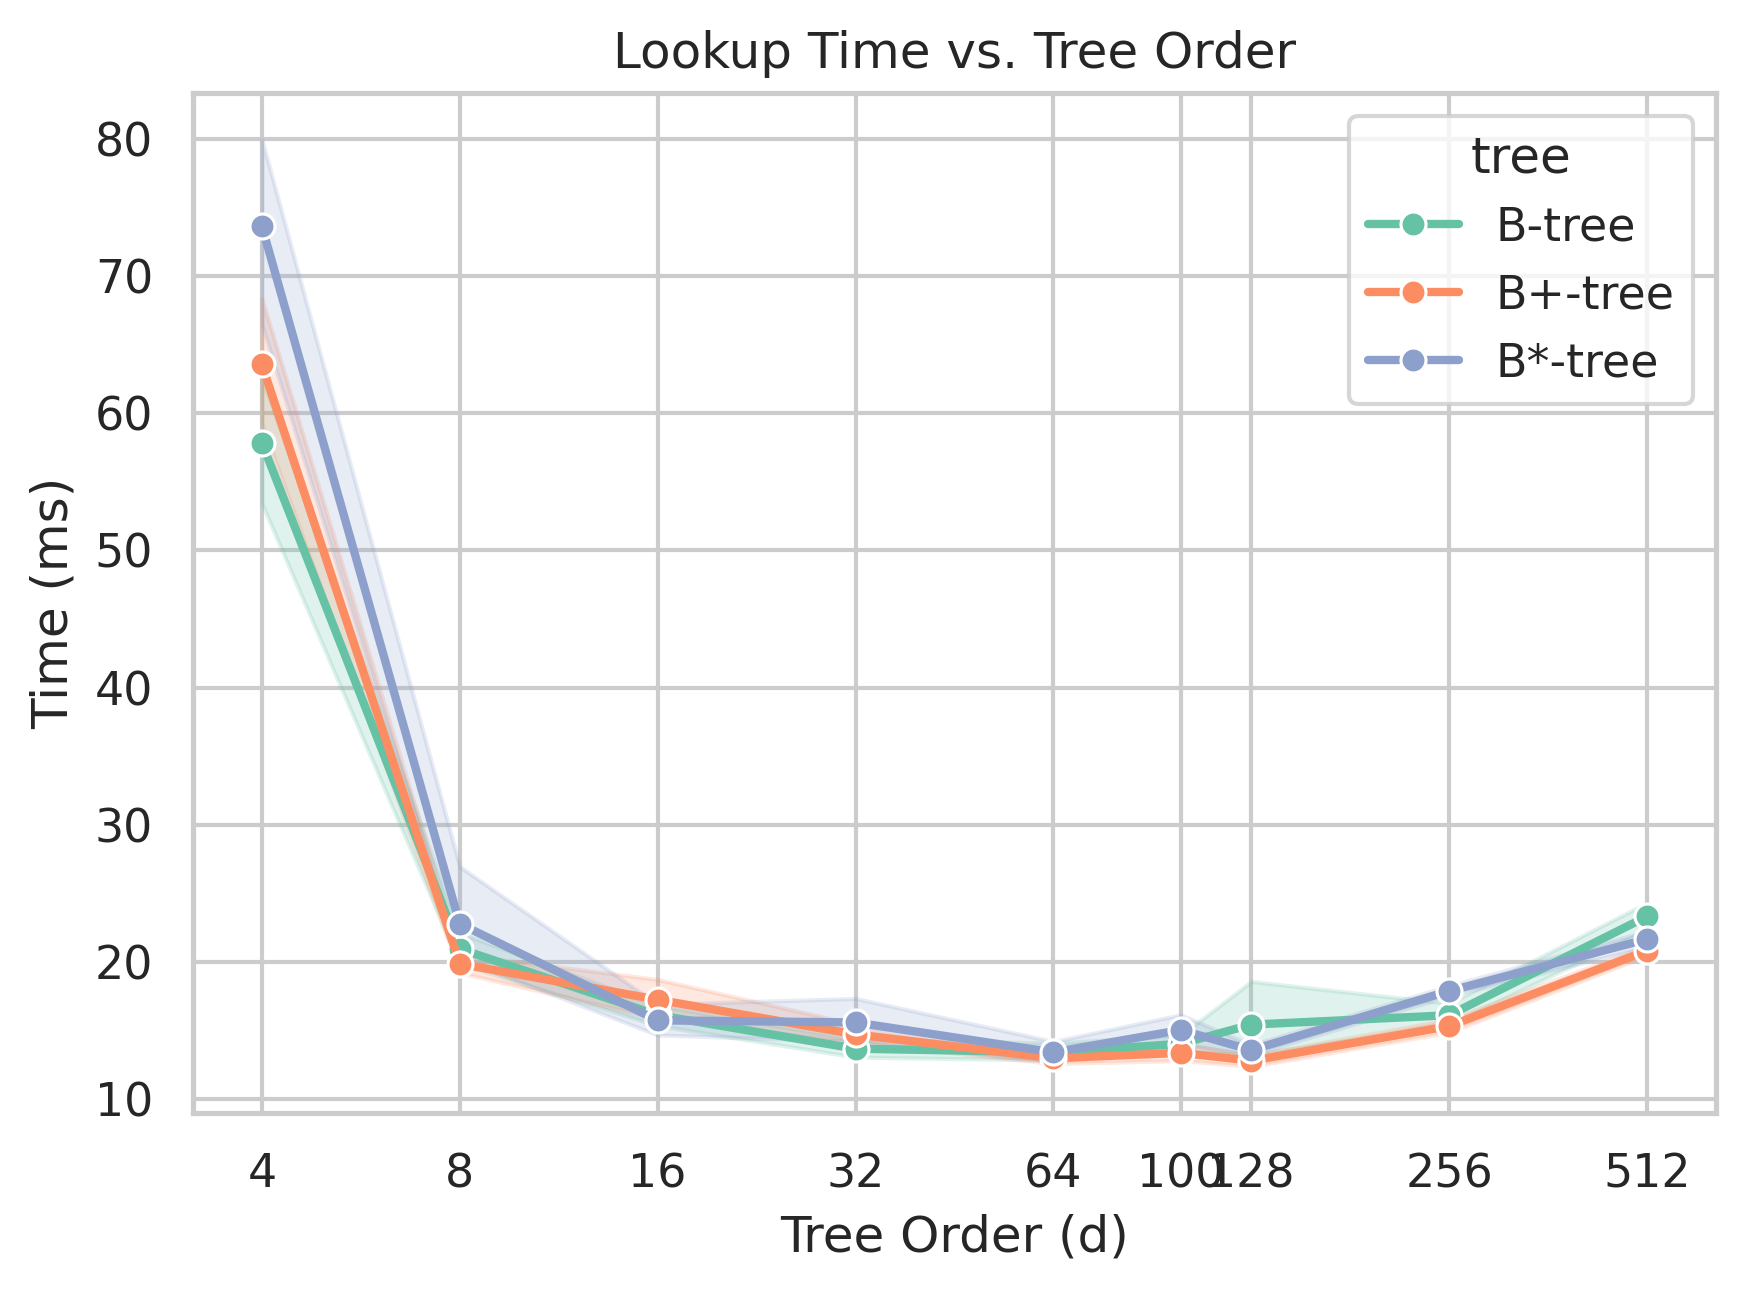
\includegraphics[width=0.7\linewidth]{figure/perf_lookup.png}
  \caption{Performance graph for searching 100000 datas}
  \label{fig:perf_lookup}
\end{figure}

All trees shows a similar performances, except for $d = 4$, where the B*-Tree performance is the worst.
B*-tree exhibits noticeably higher lookup latency compared to the other trees.
This becomes the strength of the B*-Tree because it reduces the memory usage.
However, in case of small degree, the CPU can fits the node within a single CPU cache line, the I/O benefits of the higher fill factor are removed.
Instead, extra intra-node comparison cycles results the performance decreases.

It also shows U-shaped performance curve across different orders illustrates the trade-off between tree height and intra-node operations.
The reason of U-shpae is same as insertion.


\subsection{Range query and Tree types}

\begin{figure}[H]
  \centering
  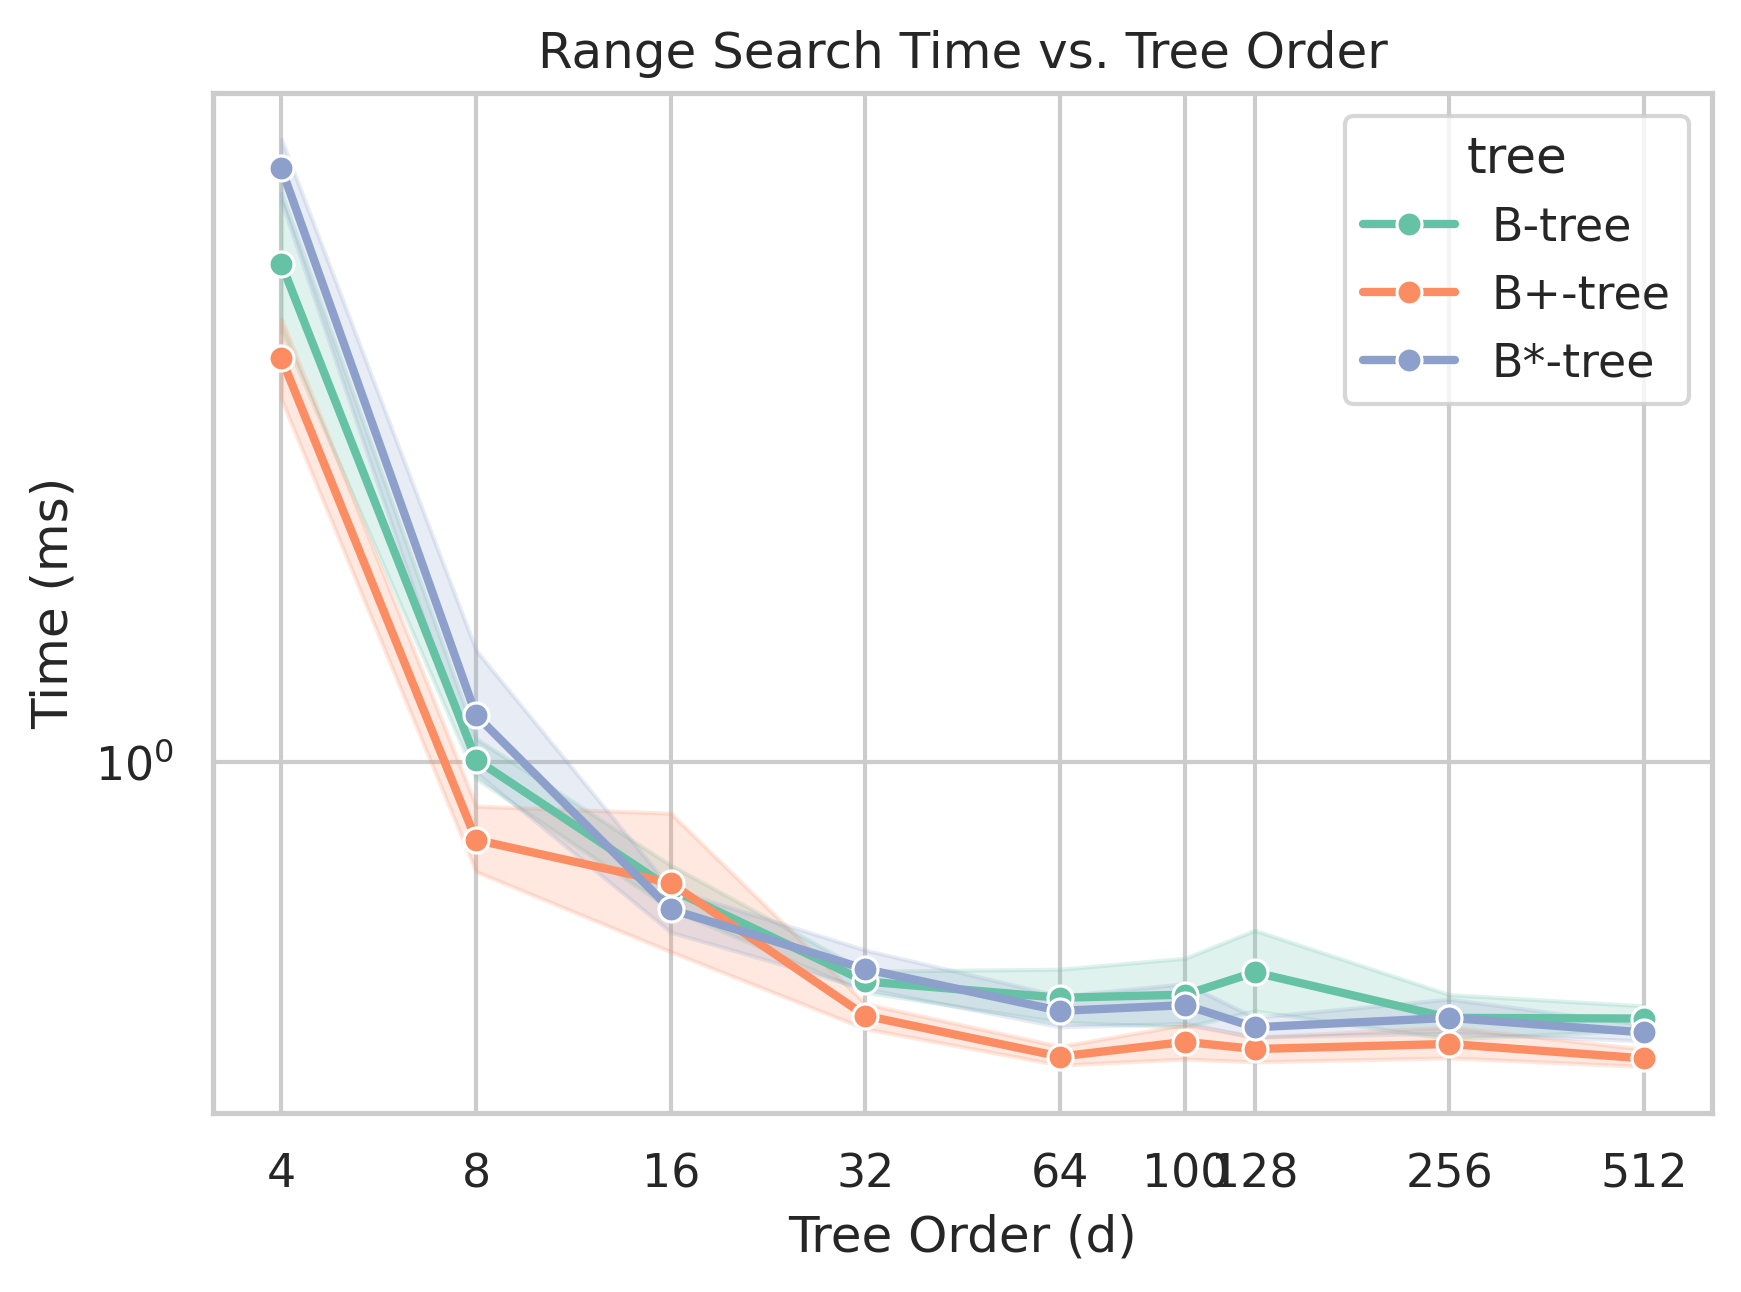
\includegraphics[width=0.7\linewidth]{figure/perf_range.png}
  \caption{Performance graph for range query}
  \label{fig:perf_range}
\end{figure}

Note that y-axis of \Cref{fig:perf_range} is log scaled.

B+-tree performs the best in almost every $d$ values while other two tree performance is similar.
This shows the property of the B+-tree which contains the datas only in the leaf nodes and links between leaf nodes.
B+-tree range operation utilizes this property to achieve faster range query in sequential manner, while other trees needs to switch between parent node and child node during range query.

The U-shaped performance curve doesn't showed in this graph.
This is because This is because range queries perform read-only sequential scans, completely bypassing the expensive $O(d)$ memory shifting operations required for node modifications.
Moreover, larger $d$ makes more keys are packed into a single node, which utilizes the CPU cache operations during range operation.

\subsection{Erase and Integrity}
\begin{figure}[H]
  \centering
  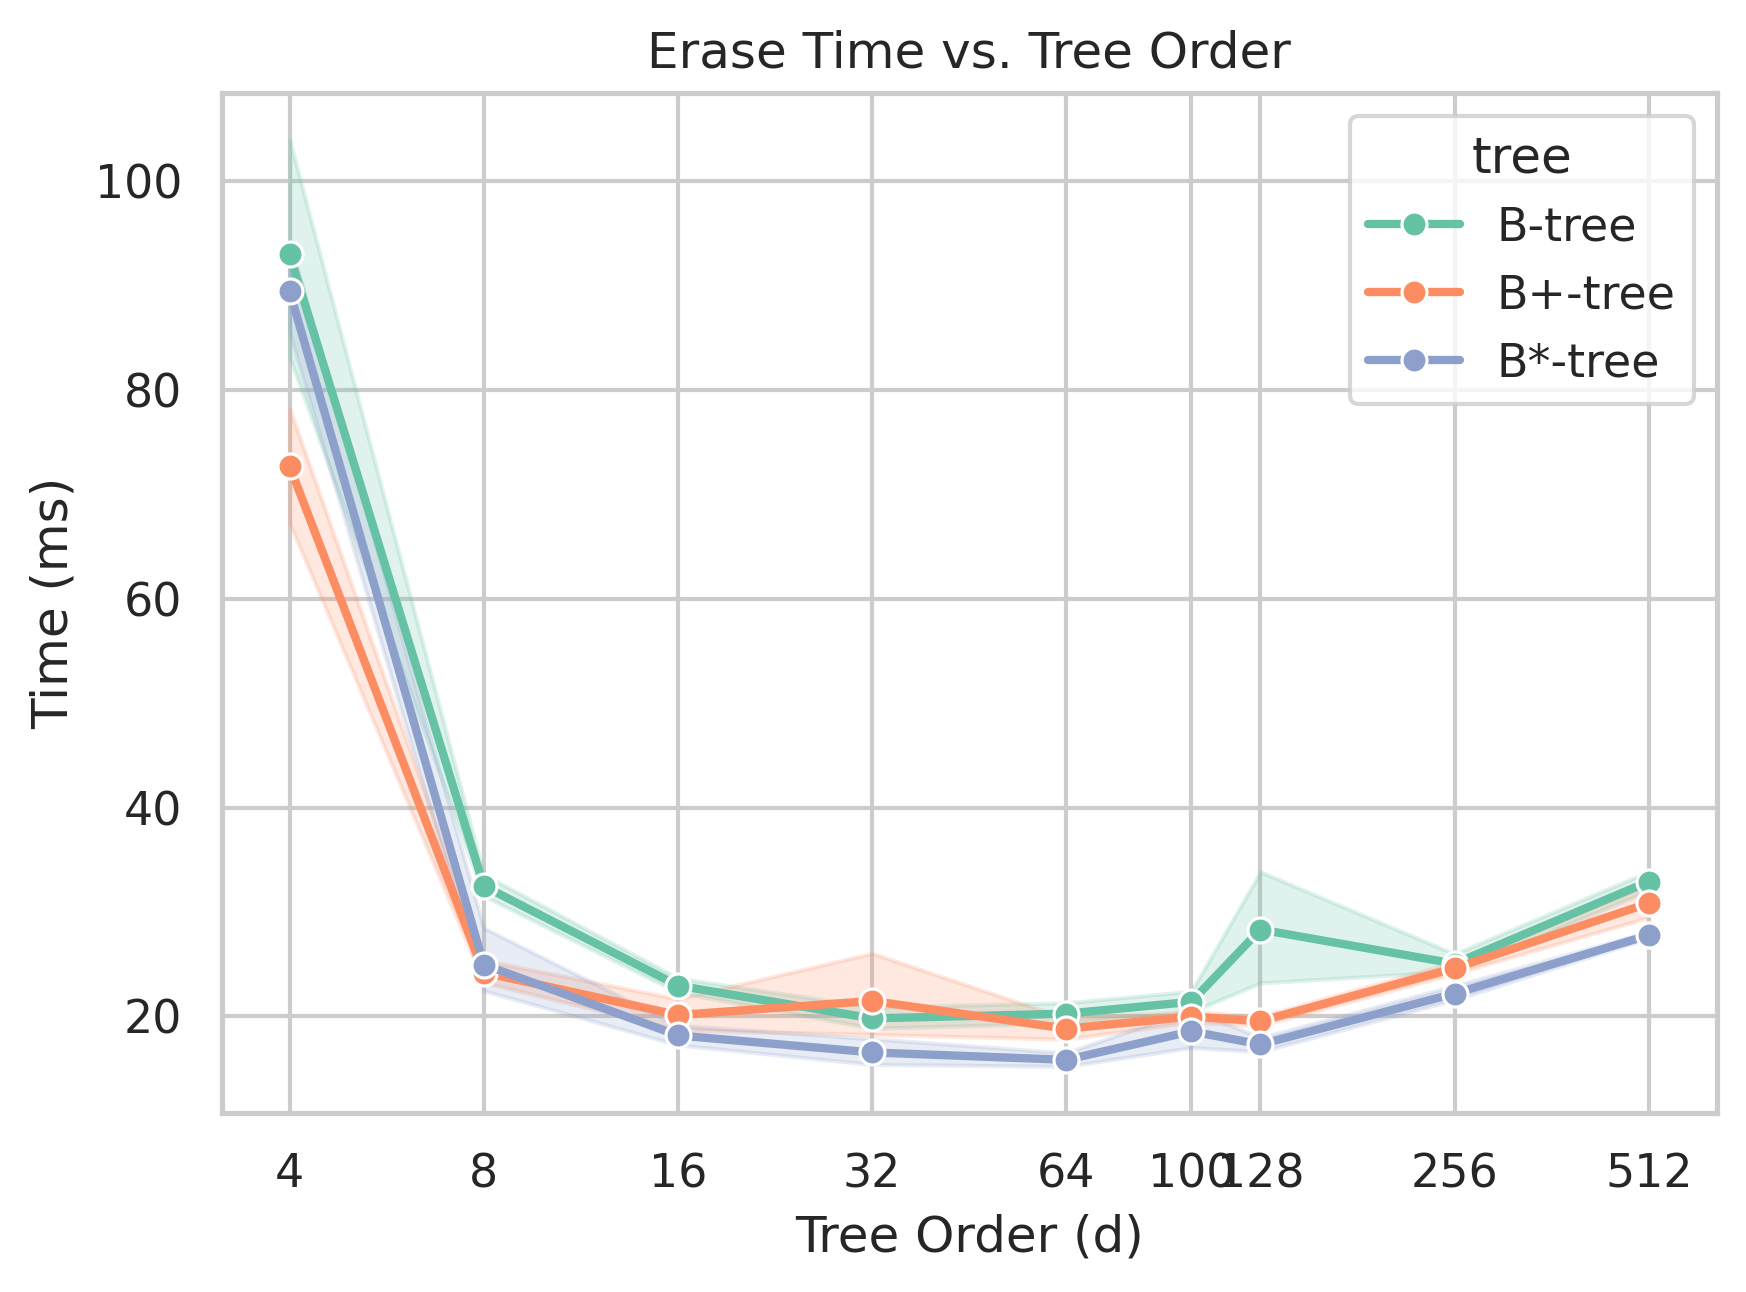
\includegraphics[width=0.7\linewidth]{figure/perf_erase.png}
  \caption{Performance graph for erase}
  \label{fig:perf_erase}
\end{figure}
As shown in \cref{fig:perf_erase}, the deletion performance forms a U-shaped curve, penalised by $O(d)$ memory shifting overhead at large orders. 
However, an interesting inversion occurs between the B*-tree and B$^+$-tree around $d=16$.

On the small degree, B+-Tree utilizes the property that it contains the actual data only at the leaf node which allows the bypass of \textit{Erase-Internal}, which contains the time consuming operation such as find succesors.
However, on large tree, although the B*-tree inherits its erase algorithm directly from the standard B-tree without a strict $3 \to 2$ merge invariant, its superior performance stems from its initial structural density.
Because B*-tree nodes hove around 66\% density, the other keys performs as `Extra Buffer' which prevents underflow.
Underflow needs a huge structual modifications such as merge, rotate, and borrow. 
By statistically avoiding expensive structural modifications (such as node rotations and merges), the B*-tree achieves the most efficient deletion times at larger orders.

For the integrity, we ran the check internal operation which check the property of the tree such as monotonically increasing keys, number of keys and children, height of leaf nodes, links on the leaf nodes in B+-Tree.
The check operation ran periodically during the erasing keys and it results zero violations.
Specifically, the internal check function was called after every 5000 deletions (10\% of the workload)
Also, we checked the cross-check between reference STL map. 
After the completion of workload, the total size, remaining keys, values are compared with STL map implementation, ensuring the implementation is algorithmically sound and robust.

\section{Additional Experiments: Insert order, Fill factor, and Height}

\begin{figure}[H]
  \centering
  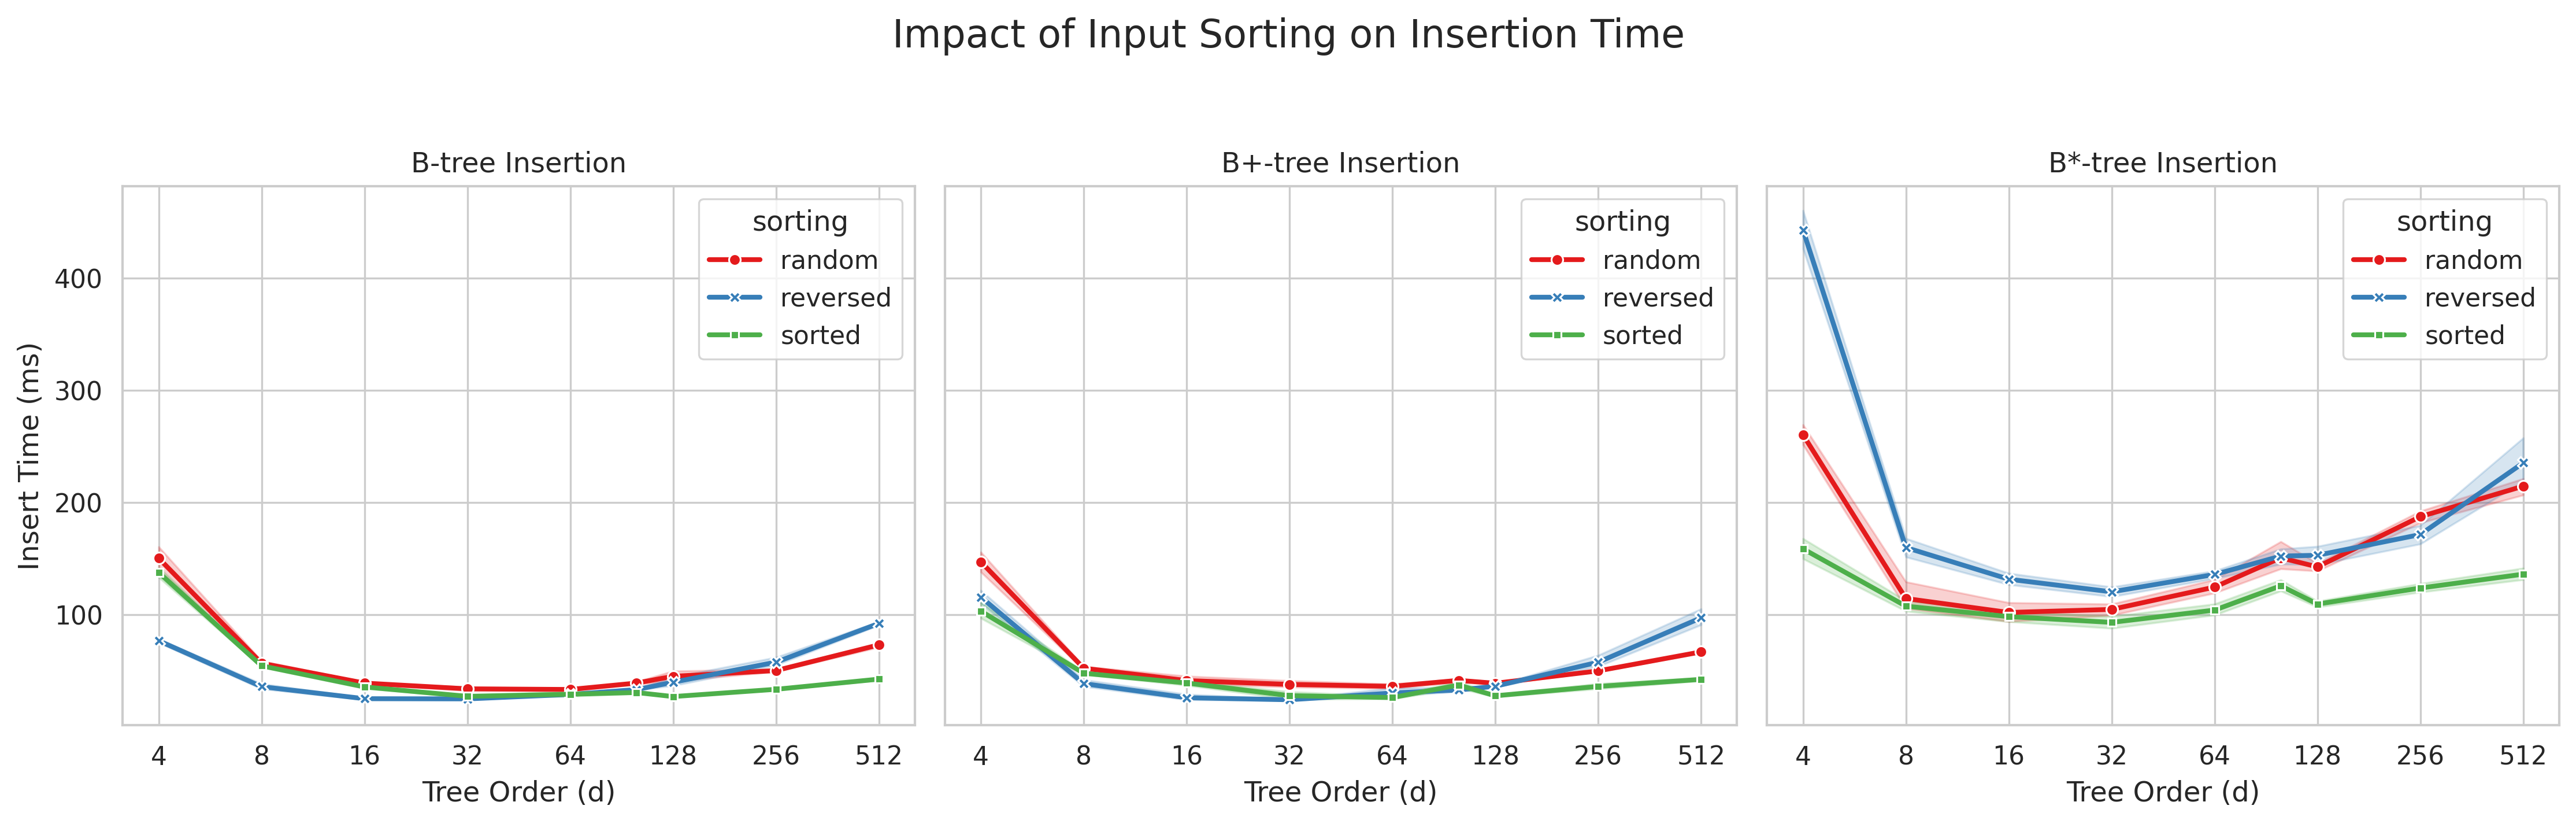
\includegraphics[width=\linewidth]{figure/insertion_sorting_analysis.png}
  \caption{Performance graph for various input order}
  \label{fig:perf_insert_sorting}
\end{figure}

Additionally, the input sorting drastically affects performance. 
Sorted inputs append to the rightmost leaf, achieving $O(1)$ cost and maximizing cache locality. 
Conversely, reversed inputs strictly insert at index 0, forcing an $O(d)$ \texttt{memmove} for every insertion, which critically degrades performance. 
At $d=4$ with reversed inputs, the B*-tree suffers severe bottlenecks as continuous index-0 insertions trigger relentless redistributions under its strict 66\% fill-factor constraint.

\begin{figure}[H]
  \centering
  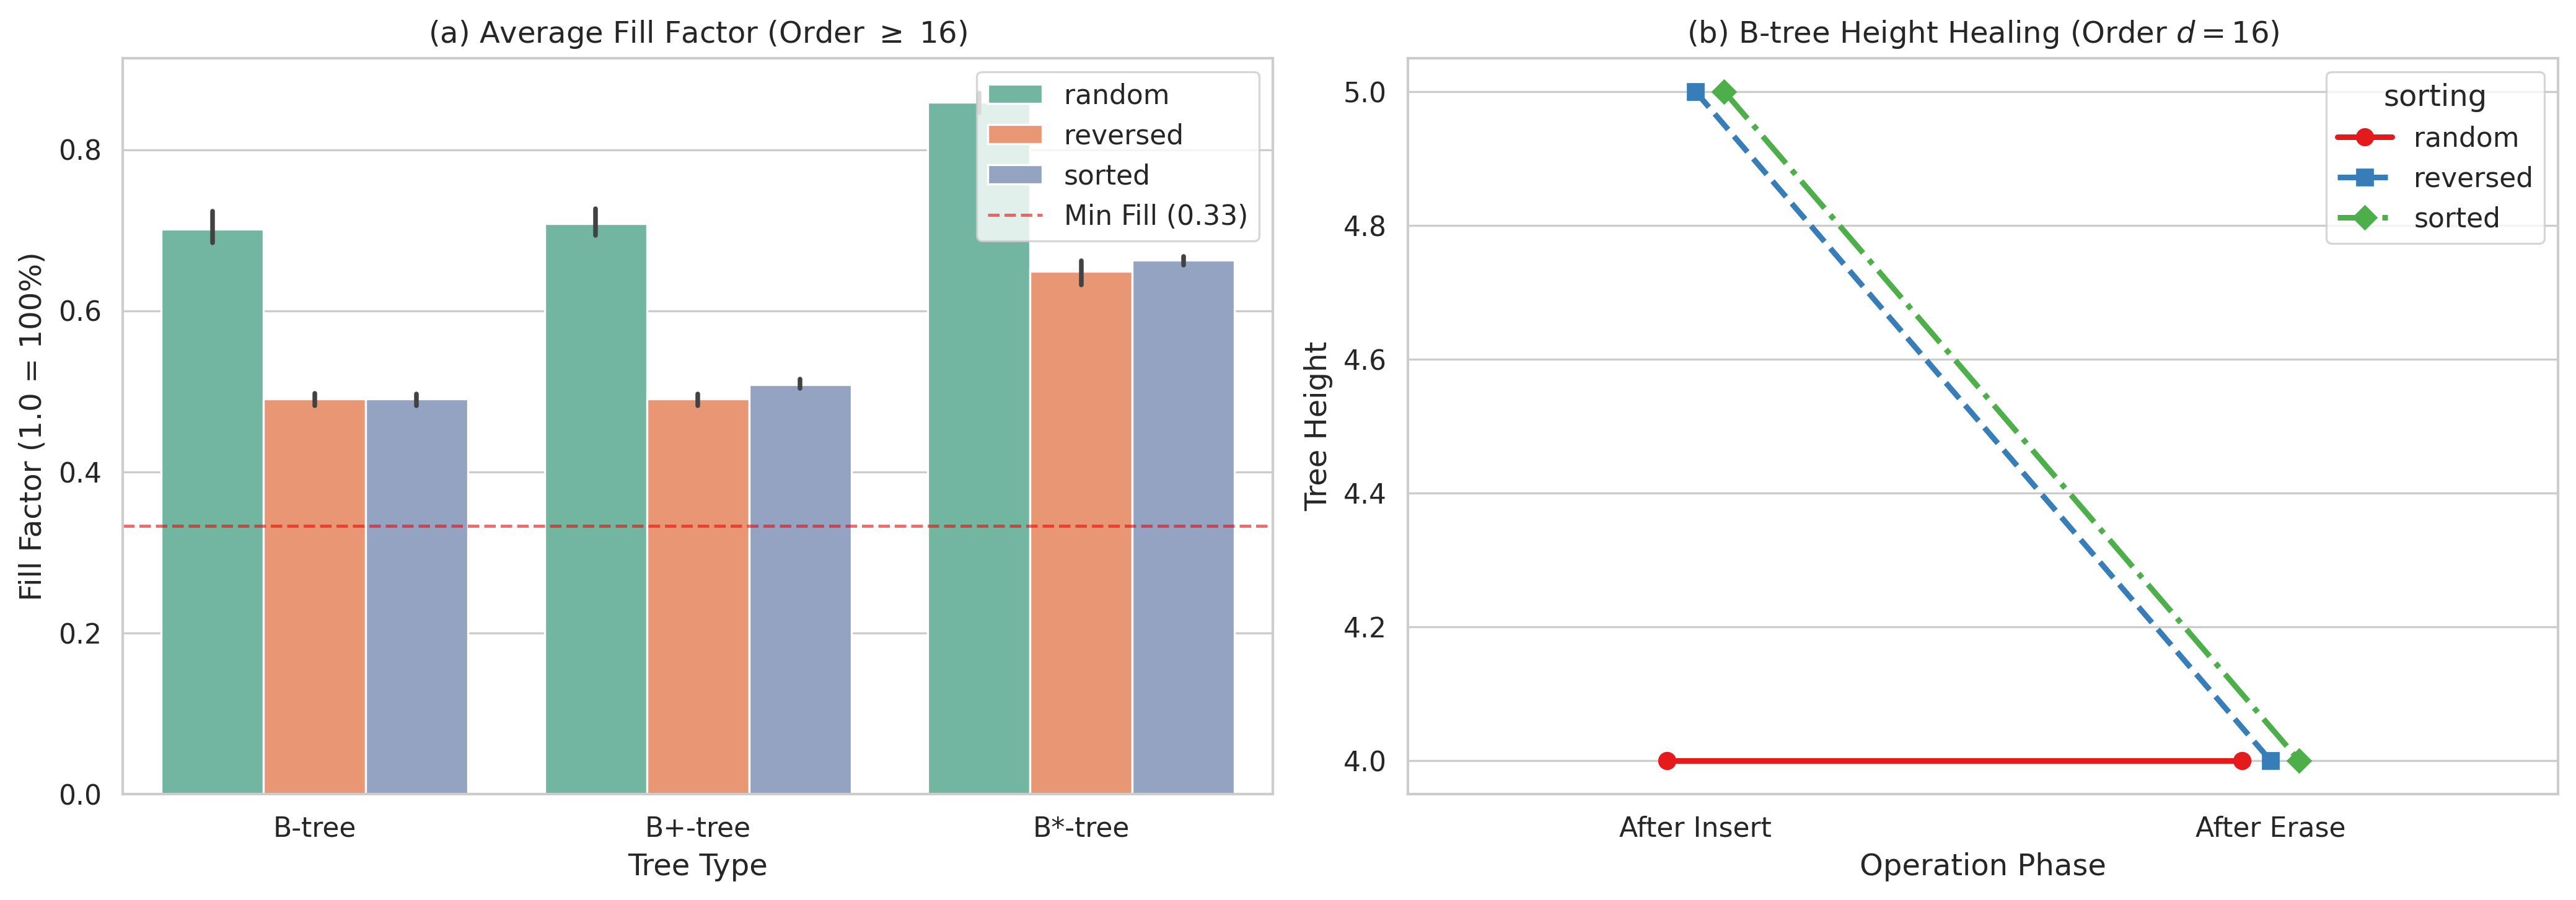
\includegraphics[width=\linewidth]{figure/integrity_combined.png}
  \caption{Fill factor and height difference}
  \label{fig:integrity}
\end{figure}

To deeply understand the B-tree variants' internal behavior, we extracted and analyzed the node fill factors and tree heights during the workloads.
As illustrated in \cref{fig:integrity}, input sorting directly dictates spatial efficiency. 
Reversed insertions cause pathological 33\% fill factors in B/B+-trees (one key per node), artificially inflating the tree height due to abandoned right-side nodes. 
Interestingly, subsequent random deletions trigger internal \textsc{Merge} operations, successfully "healing" the sparse nodes and compressing the tree back to its optimal height. 
The B*-tree, however, rigidly maintains its height and a superior $>80\%$ fill factor under random inputs, proving its structural efficiency.

\bibliographystyle{ACM-Reference-Format}
\bibliography{reference}

\end{document}